% Name: Inscribed angle theorem
% Description: The central angle on an arc is twice the inscribed angle on the same arc.
% Tags: circle theorem, inscribed angle, central angle

\usetikzlibrary{angles, quotes}

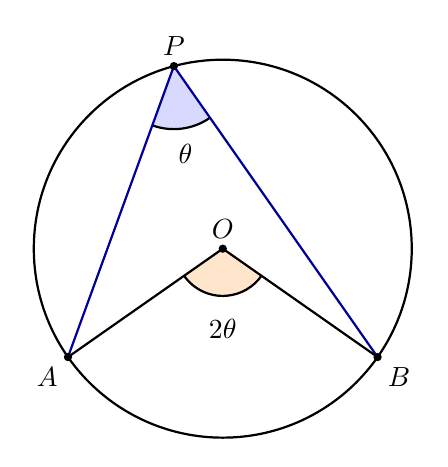
\begin{tikzpicture}[thick]
  \coordinate[label=above:$O$] (O) at (0,0);
  \coordinate[label=below left:$A$] (A) at (215:2.4);
  \coordinate[label=below right:$B$] (B) at (325:2.4);
  \coordinate[label=above:$P$] (P) at (105:2.4);
  \pic[draw, fill=orange!20, angle radius=6mm, angle eccentricity=1.7, "$2\theta$"] {angle=A--O--B};
  \pic[draw, fill=blue!15, angle radius=8mm, angle eccentricity=1.4, "$\theta$"] {angle=A--P--B};
  \draw (O) circle (2.4);
  \draw (A) -- (O) -- (B);
  \draw[blue!60!black] (A) -- (P) -- (B);
  \foreach \p in {O, A, B, P} \fill (\p) circle (1.5pt);
\end{tikzpicture}
